\documentclass[mathserif]{beamer}
\usetheme[secheader]{pecostalk}
\graphicspath{{figs/}}                                                                                                                              
\usepackage{subfigure}
\newcommand{\eqdef}{\stackrel{\text{\tiny def}}{=}}

\newcommand{\NVRvect}[1]{\ensuremath\boldsymbol{#1}}
\newcommand{\NVRtensor}[1]{\underline{\NVRvect{#1}}}
\newcommand{\NVRnorm}[1]{\left|\left|#1\right|\right|}
\newcommand{\NVRgrad}{\nabla}
\newcommand{\NVRdiv}{\NVRgrad \cdot}
\newcommand{\NVRpd}[2]{\frac{\partial#1}{\partial#2}}
\newcommand{\NVRpdd}[2]{\frac{\partial^2#1}{\partial#2^2}}
\newcommand{\NVReqdef}{\stackrel{\text{\tiny def}}{=}}

\newcommand{\NVRHgrad}{H(\text{grad})}
\newcommand{\NVRHdiv}{H(\text{div})}
\newcommand{\NVRsumm}[2]{\ensuremath\displaystyle\sum\limits_{#1}^{#2}}

\author{Jesse Chan, Nate Roberts}
\institute{The University of Texas at Austin}
\title[Camellia]{Camellia}
\subtitle{A Discontinuous Petrov-Galerkin Toolbox Using Trilinos}

\begin{document}
\begin{frame}
\begin{center}

\includegraphics[width=.8\linewidth]{grand_logo}\\
\end{center}
\titlepage
\begin{flushright}

\includegraphics[scale=0.1]{asc_logo}\\
\end{flushright}
\end{frame}

%===============================================================================
% ACKNOWLEDGEMENTS
%===============================================================================
\begin{frame}
\frametitle{Acknowledgments}

Collaborators:
\begin{itemize}
\item Leszek Demkowicz (UT/PECOS)
\item Denis Ridzal (Sandia/CSRI)
\item Pavel Bochev (Sandia/CSRI)
\end{itemize}

Support:
\begin{itemize}
\item Sandia (summer internships)
\item PECOS (GRA funding)
\item ICES (CSEM Fellowship)
\end{itemize}

\end{frame}

%===============================================================================
% From Strong-Form PDE to DPG Form
%===============================================================================
\begin{frame}                                                                                                                                                                          
\frametitle{From Strong-Form PDE to DPG Form}
\begin{center}
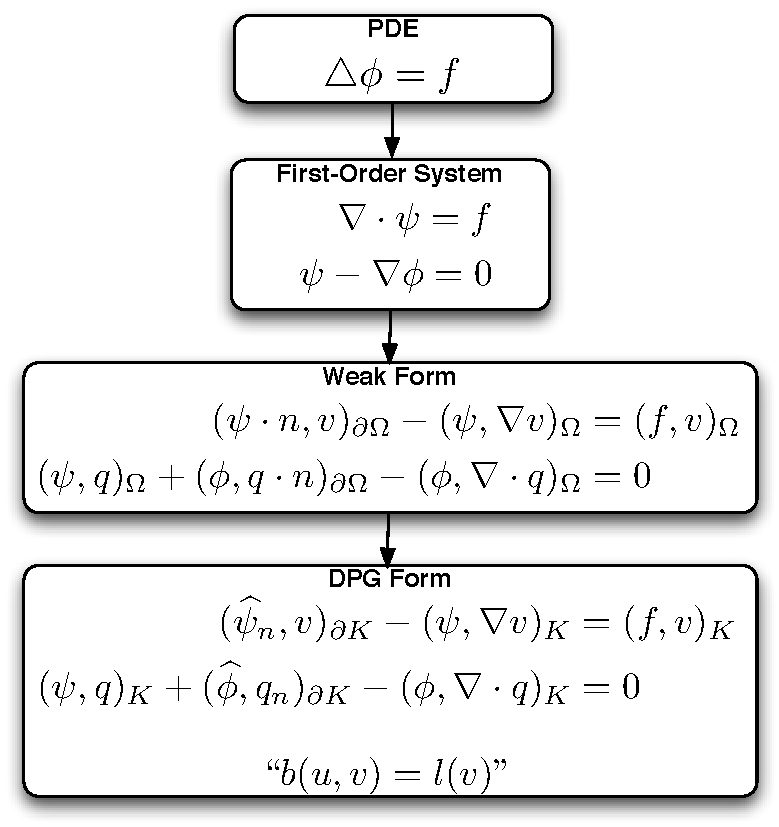
\includegraphics[width=.6\linewidth]{DPGFormCartoon}\\
\end{center}
\end{frame}              
%===============================================================================
% Solving with DPG
%===============================================================================
\begin{frame}                                                                                                                                                                          
\frametitle{Solving with DPG}
\begin{center}
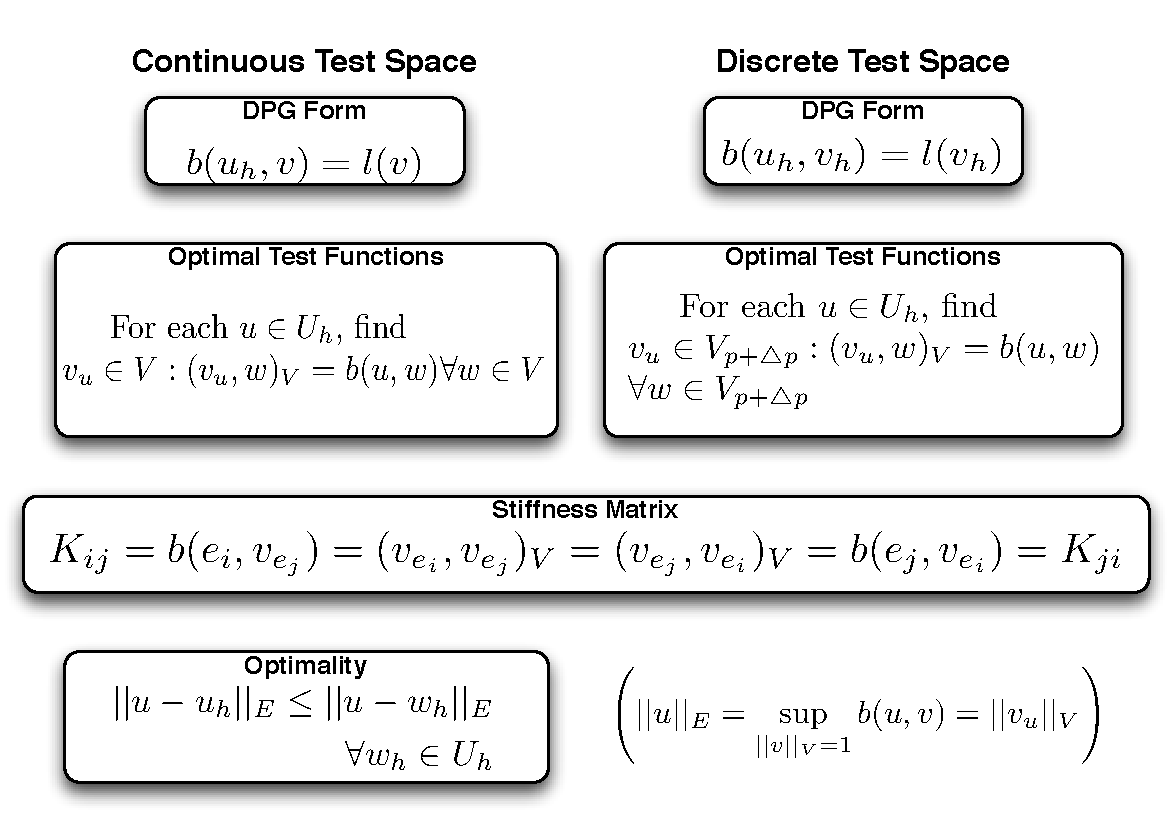
\includegraphics[width=0.9\linewidth]{DPGSolveCartoon}\\
\end{center}
\end{frame}

%===============================================================================
% CAMELLIA GOALS
%===============================================================================
\begin{frame}
\frametitle{Goals for Camellia}
\begin{block}{Goals for Camellia (Achieved)}
\begin{itemize}
\item Define $b(u,v)$ in the \emph{continuous} space (separation of concerns)
\item Arbitrary, hp-adaptive 2D meshes (quads and triangles)
\item ``Reasonable'' speed and scalability
\item Provide prebuilt versions of inner products commonly used in DPG research (mathematician's and quasi-optimal)
\end{itemize}
\end{block}

\vspace{3 mm}

\begin{block}{Goals for Camellia (Aspirational)}
\begin{itemize}
\item Support for nonlinear PDEs (Navier-Stokes in particular)
\item Better scalability (distributed solution storage, distributed mesh)
\item Longer term: 3D meshes
\end{itemize}
\end{block}

\end{frame}


%===============================================================================
% VERIFICATION APPROACH
%===============================================================================
\begin{frame}                                                                                                                                                                          
\frametitle{Camellia: Verification Approach}
\vspace {-1 mm}
\begin{block}{Unit Tests}
\begin{itemize}
\item Aspire to test-driven development.
\item Test individual features using e.g. simple PDEs, and building up from there.
\item 7095 lines of code for unit tests (compared to 10,888 for core code).
\end{itemize}
\end{block}
\begin{block}{Convergence Studies}
For Poisson and two Stokes formulations (VVP and VSP), run
\begin{itemize}
\item h-convergence studies (triangles and quads),
\item ``perverse'' p-refinement pattern on $16 \times 16$ mesh, and
\item ``hybrid'' mesh of quads and triangles.
\item 2708 lines of code for convergence studies.
\end{itemize}
\end{block}
\end{frame}

%===============================================================================
% NEW SLIDE
%===============================================================================
\begin{frame}                                                                                                                                                                          
\frametitle{Convergence Study: Stokes VSP}

\begin{table}[h!b!p!]
\begin{center}
\begin{tabular}{| c | c | c | c | c | c | c | c | c |}
\hline
\multicolumn{7}{| c |}{Stokes VSP, $u_{1}$ (triangular mesh)} \\
\hline
Mesh Size & $k=1$ & rate & $k=2$ & rate &  $k=3$ & rate \\
\hline
1 $\times$ 1		&9.4e-1	&-		&2.6e-1	&-		&5.0e-2	&-		\\
2 $\times$ 2         	&3.1e-1	&1.62	&4.3e-2	&2.63	&4.0e-3	&3.66	\\
4 $\times$ 4        	&8.0e-2	&1.94	&5.8e-3	&2.88	&2.6e-4	&3.95	\\
8 $\times$ 8         	&2.0e-2	&1.99	&7.4e-4	&2.97	&1.6e-5	&3.99	\\
16 $\times$ 16         	&5.1e-3	&2.00	&9.3e-4	&2.99	&1.0e-6	&4.00	\\
32 $\times$ 32         	&1.3e-3	&2.00	&1.2e-5	&3.00	&6.4e-8	&4.00	\\
\hline
\end{tabular}
\end{center} 
\caption{$L^{2}$ error and $h$-convergence rates for $u_{1}, k=1,2,3$.  We observe optimal convergence.}
\label{NVR:table:VSPTriRates}
\end{table}
\end{frame}

%===============================================================================
% NEW SLIDE
%===============================================================================
\begin{frame}                                                                                                                                                                          
\frametitle{Variable Polynomial Orders Study}

For this test, we used a $16 \times 16$ mesh and the following polynomial order pattern (repeated 4 times):
\\
\begin{center}
\begin{tabular}{| c | c | c | c || c | c | c | c || c | c | c | c || c | c | c | c |}
\hline
4 &4 &4 &4  &1 &1 &1 &1  &2 &2 &2 &2  &3 &3 &3 &3 \\
\hline
3 &3 &3 &3  &4 &4 &4 &4  &1 &1 &1 &1  &2 &2 &2 &2 \\
\hline
2 &2 &2 &2  &3 &3 &3 &3  &4 &4 &4 &4  &1 &1 &1 &1 \\
\hline
1 &1 &1 &1  &2 &2 &2 &2  &3 &3 &3 &3  &4 &4 &4 &4 \\
\hline
\end{tabular}
\end{center}
\end{frame}

%===============================================================================
% NEW SLIDE
%===============================================================================
\begin{frame}                                                                                                                                                                          
\frametitle{Variable Polynomial Orders Study, Poisson Results}
\begin{center}
\begin{tabular}{| c | c | c | c | c | c |}
\hline
\multicolumn{6}{| c |}{Triangles} \\
\hline
\multicolumn{2}{| c |}{$\phi$} & \multicolumn{2}{| c |}{$\psi_{1}$} & \multicolumn{2}{| c |}{$\psi_{2}$} \\
\hline
$k=1$ & mixed $k$ & $k=1$ & mixed $k$ & $k=1$ & mixed $k$ \\
\hline
2.0e-3 & 9.1e-4 & 3.4e-3 & 1.7e-3 & 2.4e-3 & 1.1e-3\\
\hline
\hline
\multicolumn{6}{| c |}{Quads} \\
\hline
\multicolumn{2}{| c |}{$\phi$} & \multicolumn{2}{| c |}{$\psi_{1}$} & \multicolumn{2}{| c |}{$\psi_{2}$} \\
\hline
$k=1$ & mixed $k$ & $k=1$ & mixed $k$ & $k=1$ & mixed $k$ \\
\hline
1.0e-3 & 3.7e-4 & 2.3e-3 & 6.6e-4 & 2.9e-3 &1.2e-3\\
\hline
\end{tabular}
\end{center}
\end{frame}

%===============================================================================
% NEW SLIDE
%===============================================================================
\begin{frame}
\frametitle{Poisson Manufactured Solution, ``Hybrid'' Cubic Mesh}
\begin{columns}[c]
\begin{column}{5.5cm}
\begin{block}{$\phi$}
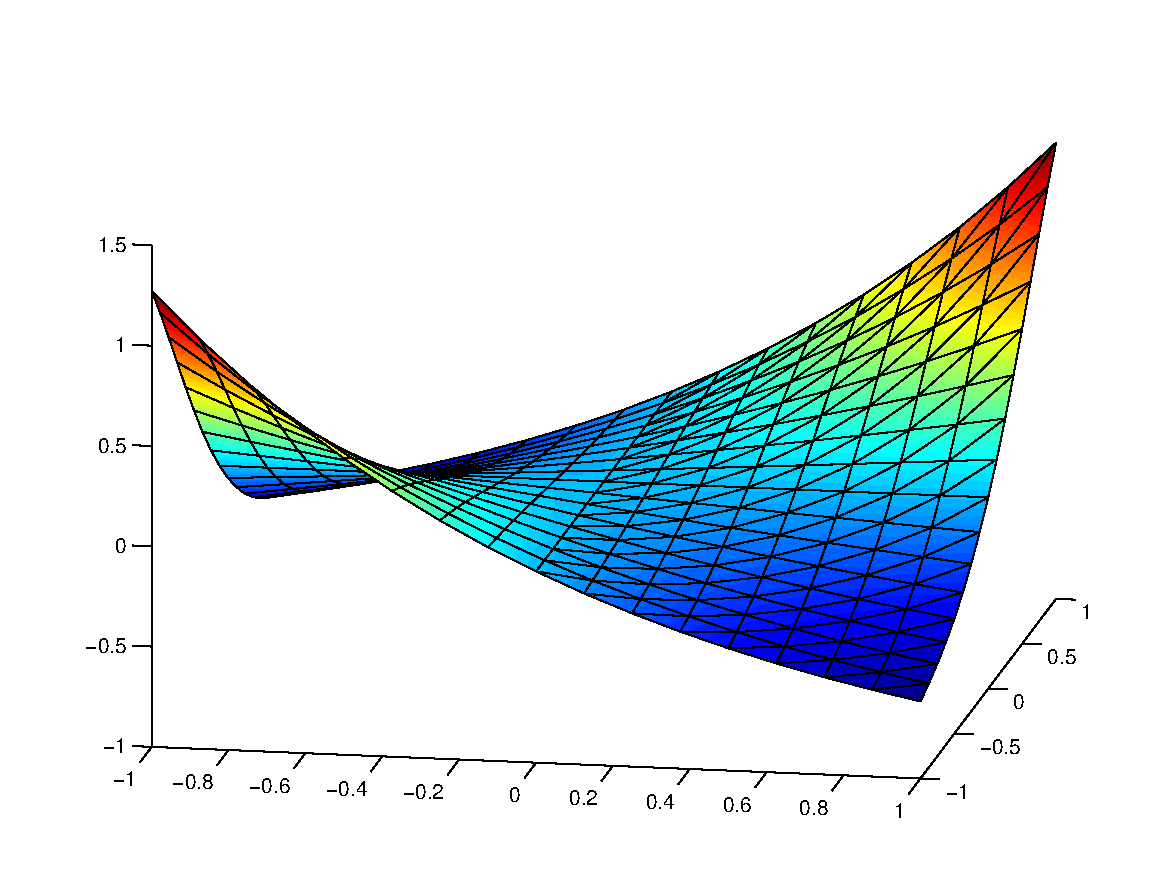
\includegraphics[width=5.5cm]{phicubic16x16}
\end{block}
\end{column}
\begin{column}{5.5cm}
\begin{block}{$\psi_{1}$}
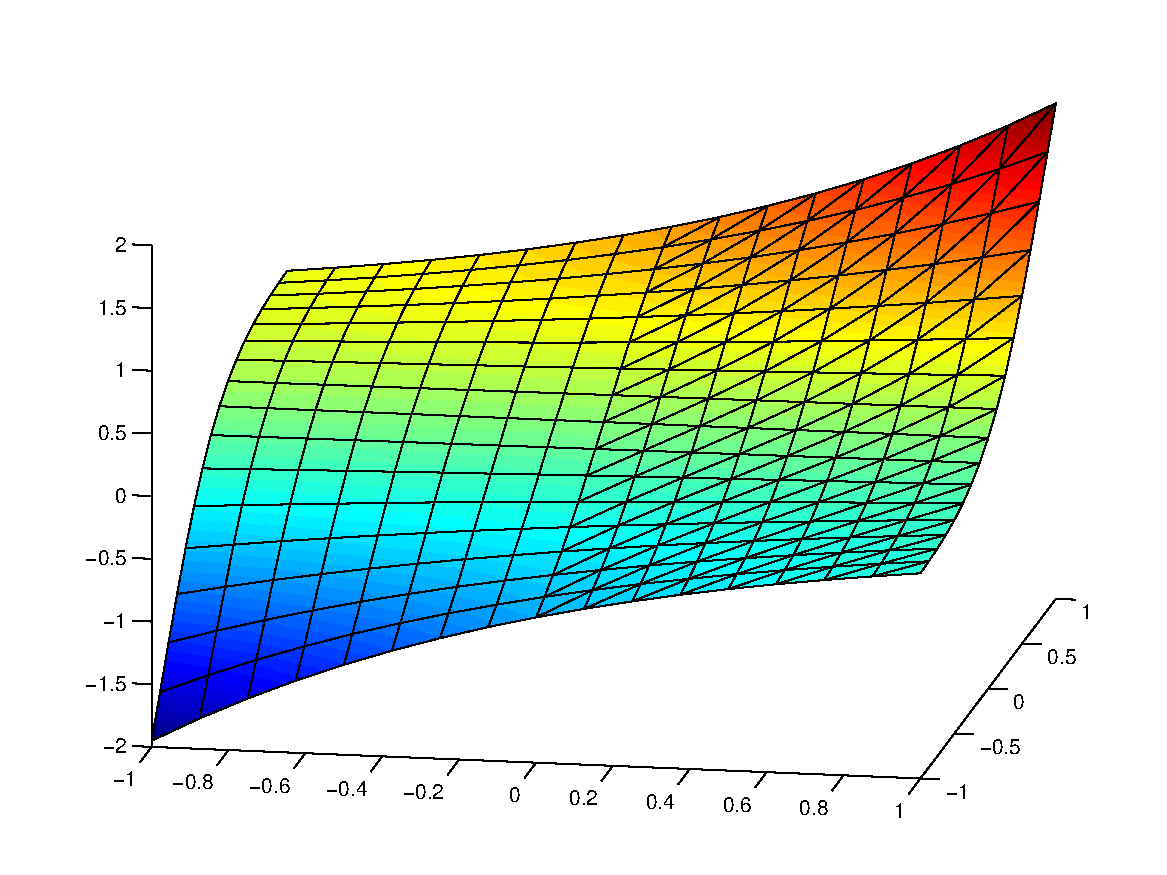
\includegraphics[width=5.5cm]{psi1cubic16x16}
\end{block}
\end{column}
\end{columns}
\end{frame}


%===============================================================================
% NEW SLIDE
%===============================================================================
\begin{frame}
\frametitle{Stokes Manufactured Solution, ``Hybrid'' Cubic Mesh}
\begin{columns}[c]
\begin{column}{5.5cm}
\begin{block}{Pressure}
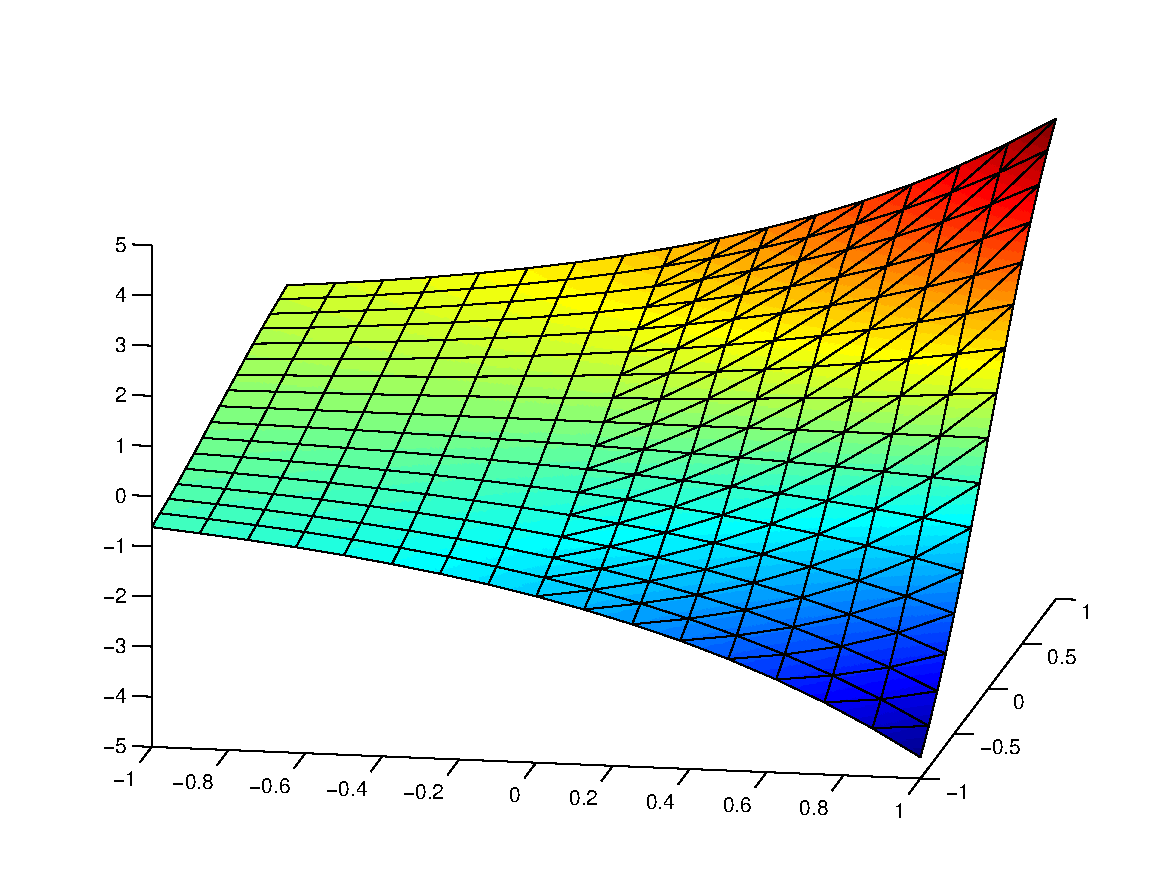
\includegraphics[width=5.5cm]{pressurecubic16x16}
\end{block}
\end{column}
\begin{column}{5.5cm}
\begin{block}{Velocity ($y$ component)}
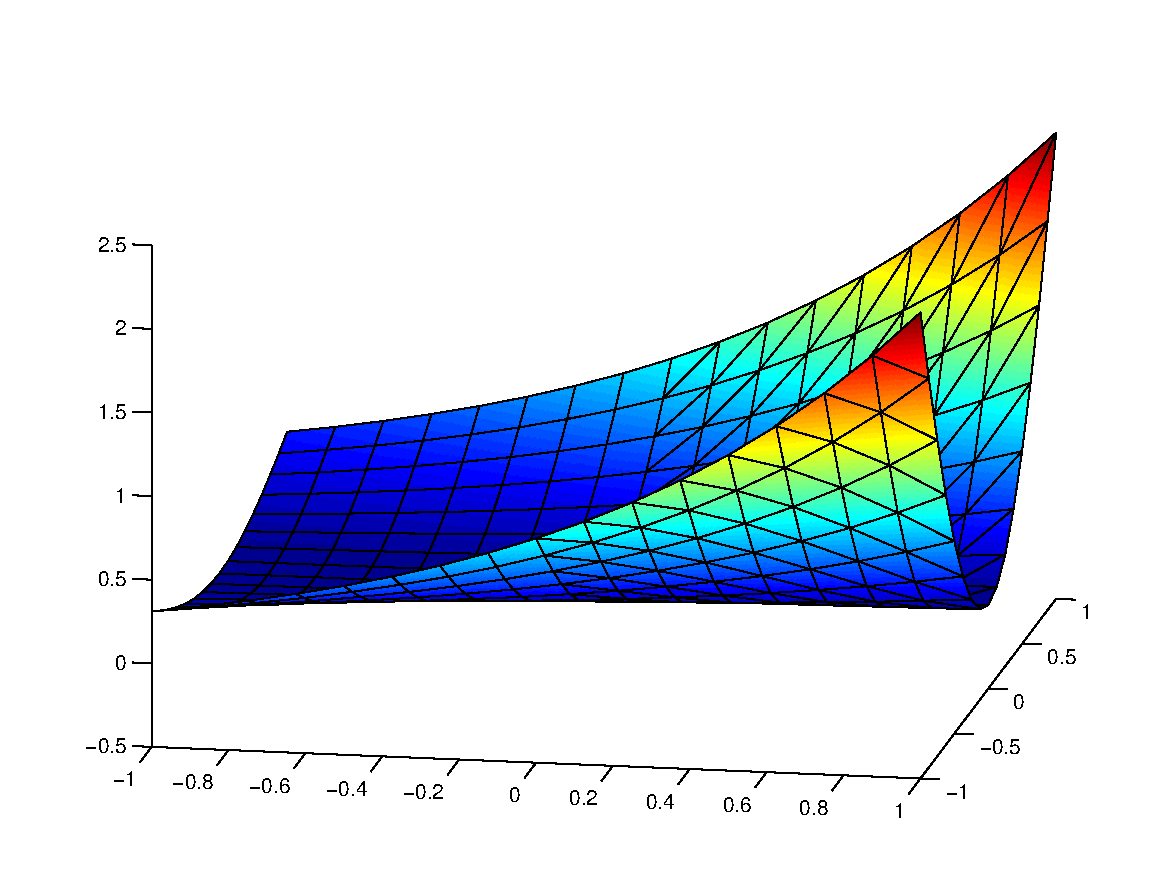
\includegraphics[width=5.5cm]{u2cubic16x16}
\end{block}
\end{column}
\end{columns}
\vspace{3 mm}
\end{frame}

%===============================================================================
% Jesse's projects
%===============================================================================

\begin{frame}
\frametitle{New proof of robustness in $\epsilon$}

\begin{columns}[c]
\begin{column}{5.5cm}
\begin{block}{Solution variable $u$}
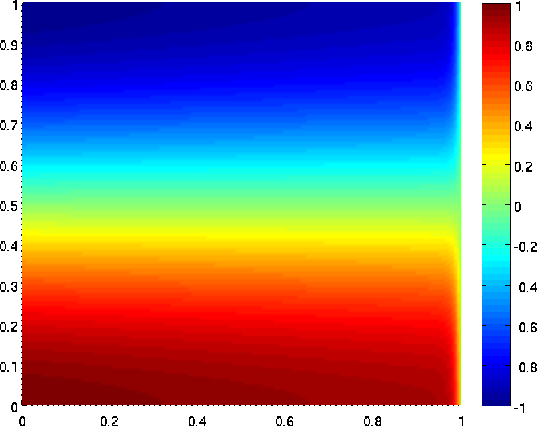
\includegraphics[width=5.5cm]{../../jesse/FERodeo2012/figs/wallBC_exact_u.png}
\end{block}
\end{column}
\begin{column}{5.4cm}
\begin{block}{$L^2$ error}
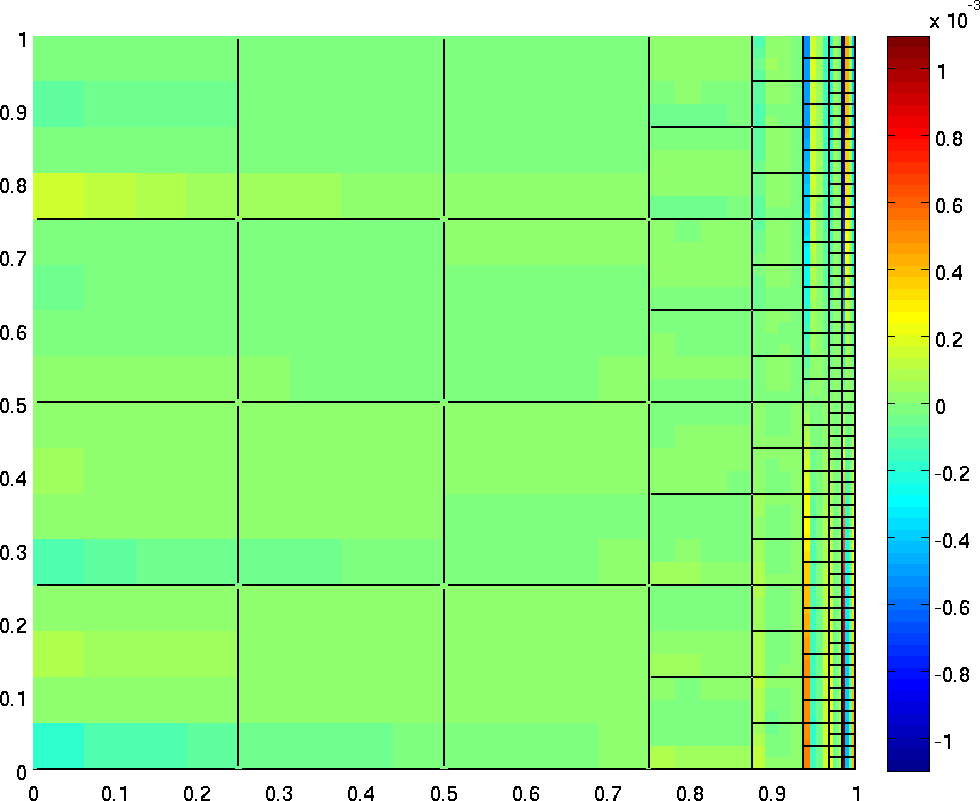
\includegraphics[width=5.4cm]{../../jesse/FERodeo2012/figs/u_pointdiff_wallBC.png}
\end{block}
\end{column}
\end{columns}
\vspace{3 mm}

Solution/pointwise error in $u$ for inflow boundary condition on $\beta_n u - \sigma_n$.  Method is provably robust (quality does not degenerate with $\epsilon \rightarrow 0$)

\end{frame}

\begin{frame}
\frametitle{New proof of robustness in $\epsilon$}

\begin{columns}[c]
\begin{column}{5.5cm}
\begin{block}{Solution variable $u$}
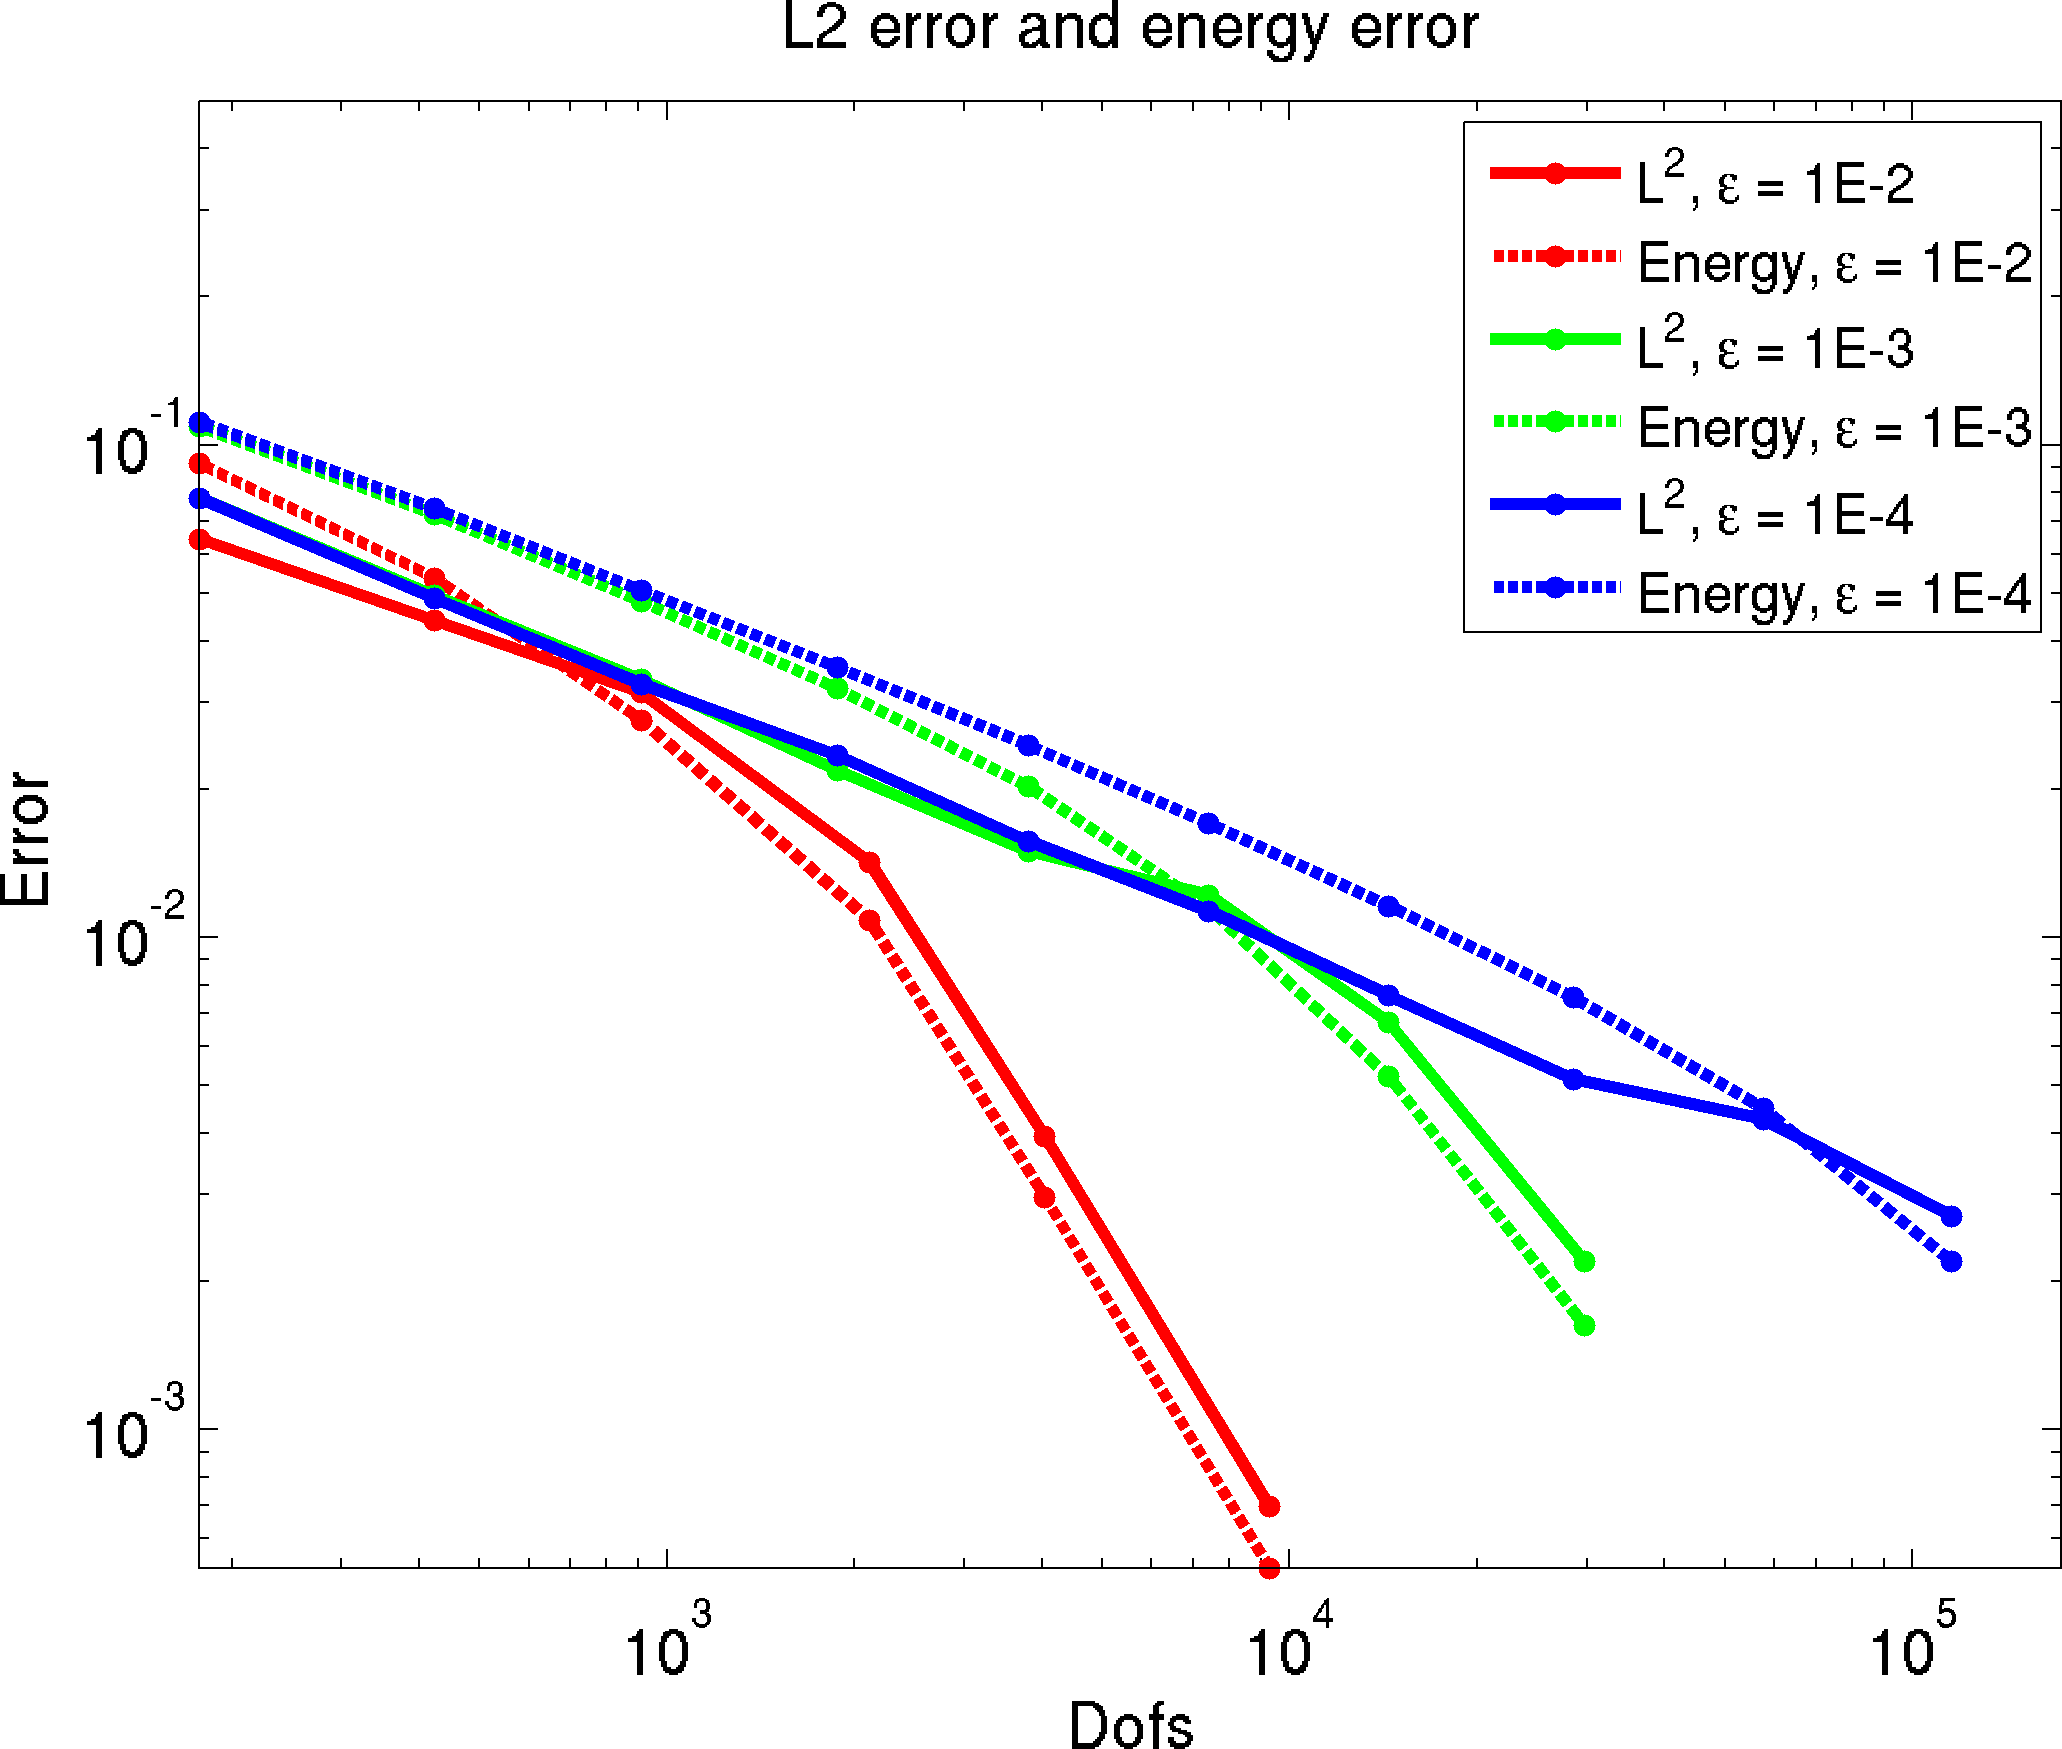
\includegraphics[width=5.5cm]{../../jesse/FERodeo2012/figs/errorrates_wallBC.png}
\end{block}
\end{column}
\begin{column}{5.4cm}
\begin{block}{$L^2$ error}
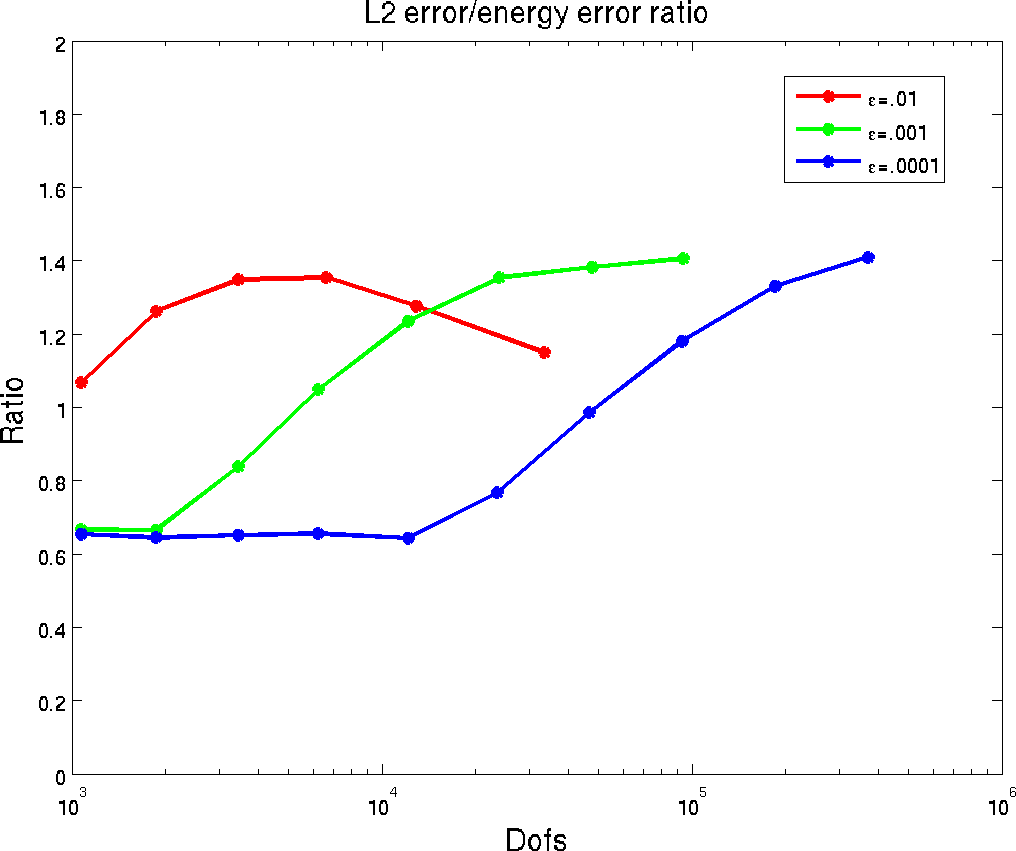
\includegraphics[width=5.4cm]{../../jesse/FERodeo2012/figs/L2energyratio_wallBC.png}
\end{block}
\end{column}
\end{columns}
\vspace{3 mm}

$L^2$ and energy error comparison, and the ratio of $L^2$ to energy error for inflow boundary condition on $\beta_n u - \sigma_n$.  Solution is nearly identical to the $L^2$ projection for wide range of $\epsilon$. 

\end{frame}


\begin{frame}
\frametitle{Regularization using small diffusion}

\begin{columns}[c]
\begin{column}{5.5cm}
\begin{block}{Solution variable $u$}
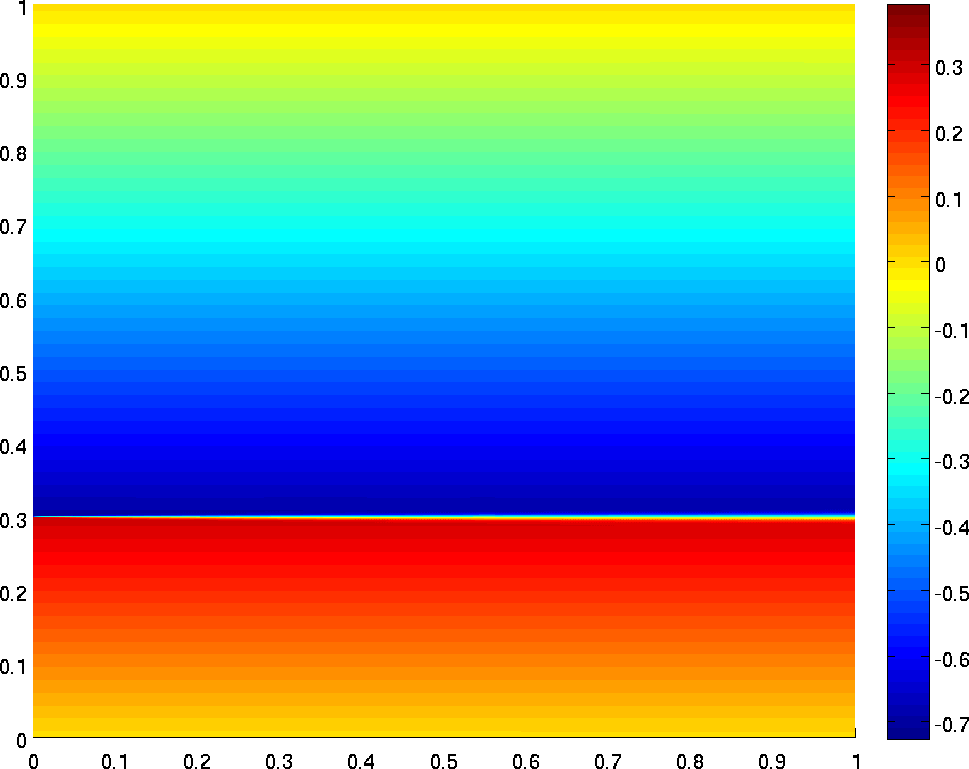
\includegraphics[width=5.5cm]{../../jesse/FERodeo2012/figs/discontinuous.png}
\end{block}
\end{column}
\begin{column}{5.5cm}
\begin{block}{$L^2$ pure convection error}
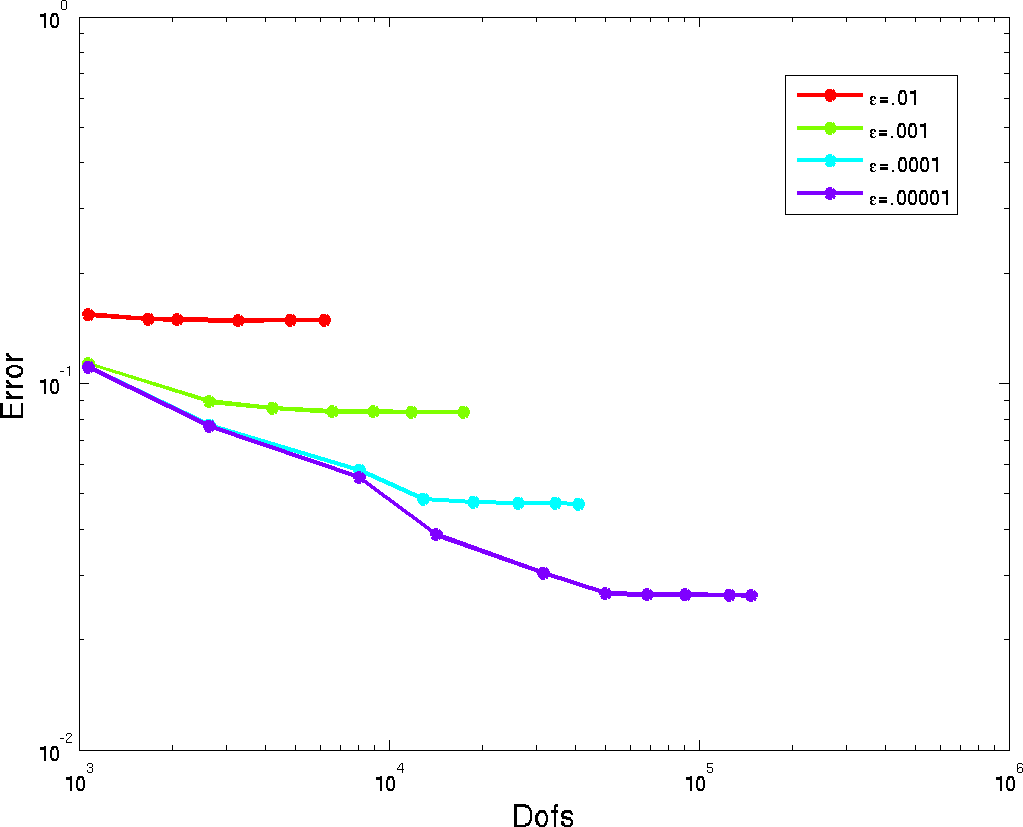
\includegraphics[width=5.5cm]{../../jesse/FERodeo2012/figs/discontinuousL2rates.png}
\end{block}
\end{column}
\end{columns}
\vspace{3 mm}

Convection of a discontinuous hat, regularized by small diffusion $\epsilon = 1e-5$.  Unaligned with the mesh (worst case scenario).  

\end{frame}

\begin{frame}
\frametitle{Regularization of ill-posed convection problems}

\begin{columns}[c]
\begin{column}{5.5cm}
\begin{block}{Solution variable $u$}

\includegraphics[width=5.5cm]{../../jesse/FERodeo2012/figs/vortex.png}
\end{block}
\end{column}
\begin{column}{5.5cm}
\begin{block}{Mesh after 5 refinement steps}
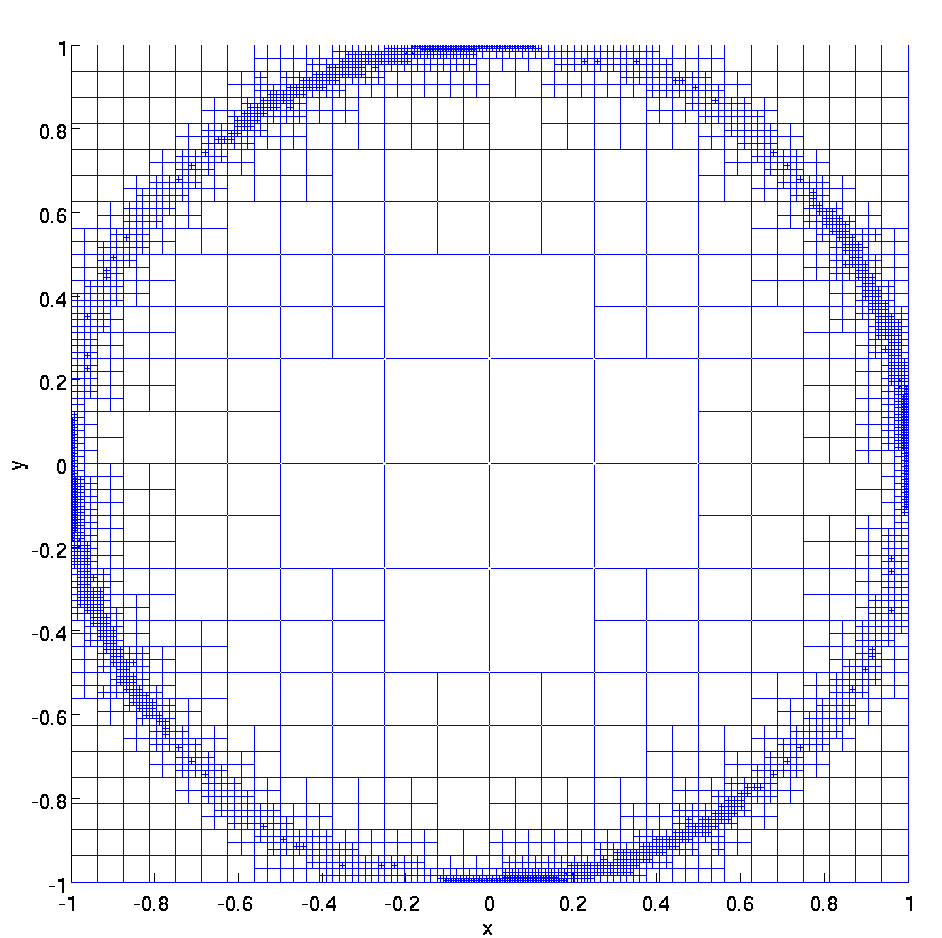
\includegraphics[width=5.5cm]{../../jesse/FERodeo2012/figs/vortexMesh.png}
\end{block}
\end{column}
\end{columns}
\vspace{3 mm}

Vorticular convection problem with $\beta = (-y,x)$, regularized with $\epsilon=1e-5$.  Ill-posed in the convection setting.

\end{frame}



%===============================================================================
% CURRENT AND FUTURE WORK
%===============================================================================
\begin{frame}
\frametitle{Current and Future Work}
\begin{block}{}
\begin{itemize}
\item Nonlinear PDE support
\item Better scalability (distributed mesh and solution storage)
\item Application to Navier-Stokes
\end{itemize}
\end{block}

\begin{columns}[c]
\begin{column}{5.5cm}
\begin{block}{Convection-Diffusion, $\epsilon=10^{-2}$}
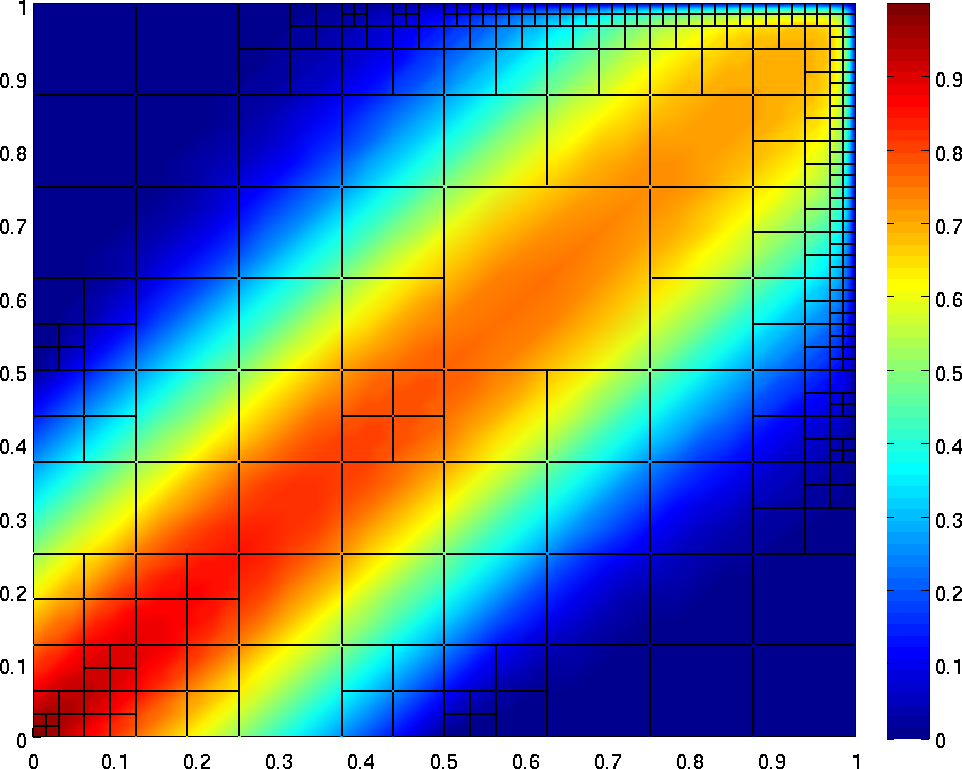
\includegraphics[width=5.5cm]{../../jesse/BoardOfVisitors/BOVslide/confusionDemo.png}
\end{block}
\end{column}
\begin{column}{5.5cm}
\begin{block}{Burgers', $\epsilon=10^{-4}$}
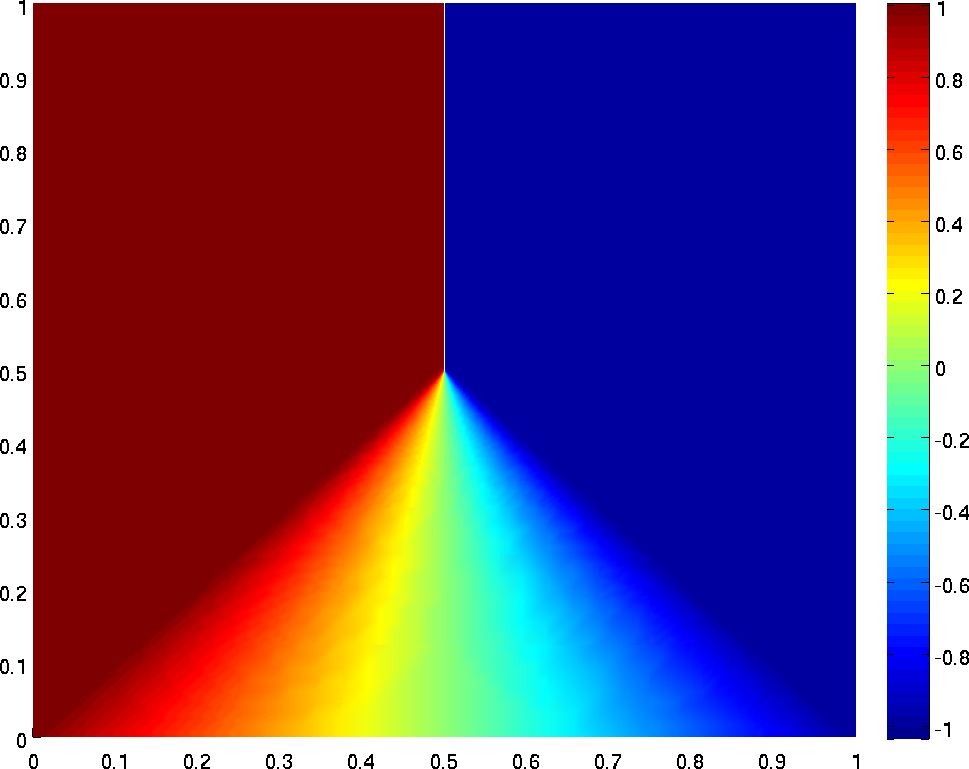
\includegraphics[width=5.5cm]{burgers1e4.png}
\end{block}
\end{column}
\end{columns}
\end{frame}


%===============================================================================
% NEW SLIDE
%===============================================================================
\begin{frame}
\frametitle{}
\begin{block}{}
For more info on Camellia:\\
\{nroberts, jchan985\}@ices.utexas.edu\\
\url{https://cfwebprod.sandia.gov/cfdocs/CCIM/docs/Roberts_et_al_SAND2011-6678.pdf}
\end{block}

\end{frame}

 
\end{document}
